% IEEEtran journal-style typesetting sample.
% The observations and research scenario in this paper are synthetic.
% Build from the repository root with: make paper
\documentclass[journal]{IEEEtran}

\usepackage{amsmath,amssymb,amsfonts,bm}
\usepackage{mathtools}
\usepackage{graphicx}
\usepackage{subcaption}
\usepackage{booktabs}
\usepackage{siunitx}
\usepackage{xcolor}
\usepackage{tikz,pgfplots}
\usetikzlibrary{positioning,arrows.meta,calc,fit,backgrounds,automata}
\pgfplotsset{compat=1.17}
\usepackage{cite}
\usepackage[hidelinks]{hyperref}
\usepackage[capitalise,noabbrev]{cleveref}

\DeclareMathOperator*{\argmin}{arg\,min}
\DeclareMathOperator{\softmax}{softmax}
\DeclareMathOperator{\Var}{Var}
\DeclareMathOperator{\Cov}{Cov}
\DeclareMathOperator{\tr}{tr}
\newcommand{\E}{\mathbb{E}}
\newcommand{\R}{\mathbb{R}}
\DeclareSIUnit\gforce{\textit{g}}
\sisetup{detect-weight=true, detect-family=true}

% ---------------------------------------------------------------
% Shared TikZ styles. Fonts are inherited from the host document,
% so labels match the body text automatically (no hard-coded fonts).
% Required: \usepackage{tikz,pgfplots}, \usetikzlibrary{positioning,
%   arrows.meta,calc,fit,backgrounds,automata,shapes.geometric}
% ---------------------------------------------------------------
\definecolor{oiBlue}{HTML}{0072B2}
\definecolor{oiOrange}{HTML}{E69F00}
\definecolor{oiGreen}{HTML}{009E73}
\definecolor{oiVerm}{HTML}{D55E00}
\definecolor{oiSky}{HTML}{56B4E9}

\tikzset{
  >={Stealth[length=1.6mm]},
  every node/.append style={font=\footnotesize},
  block/.style={draw, rounded corners=1pt, minimum width=22mm, minimum height=6.5mm,
                align=center, line width=0.5pt, inner sep=2pt},
  attn/.style={block, fill=oiBlue!15, draw=oiBlue!80!black},
  ffn/.style={block, fill=oiGreen!15, draw=oiGreen!60!black},
  norm/.style={block, fill=oiOrange!18, draw=oiOrange!70!black, minimum height=5mm},
  embed/.style={block, fill=oiSky!20, draw=oiSky!60!black},
  head/.style={block, fill=oiVerm!12, draw=oiVerm!70!black},
  flow/.style={->, line width=0.5pt},
  skip/.style={->, line width=0.5pt, dashed, oiVerm!80!black},
  sum/.style={circle, draw, inner sep=0.8pt, line width=0.5pt},
  state/.style={circle, draw, minimum size=9mm, line width=0.5pt, inner sep=1pt},
  accepting/.style={double, double distance=1pt},
}

\graphicspath{{../../figures/}}
\input{../../figures/key_numbers}

\begin{document}

\title{Temperature and Power in a Synthetic Sensor Dataset: A Typesetting Demonstration}

\author{Muhammad Uzair Javed%
\thanks{This paper is a portfolio typesetting example. The observations are synthetic and do not represent a real monitoring site. Source: \url{https://github.com/uzairjaved-prog/Academic-typesetting-portfolio}.}}

\markboth{JOURNAL PAPER SAMPLE (PORTFOLIO DEMONSTRATION)}{Javed: Temperature and Power in Example Data}
\maketitle

\begin{abstract}
This paper demonstrates an IEEE-style workflow using 2,880 synthetic hourly observations from three example sites. A hinge regression is fitted by least squares, with its threshold selected by a grid search. The in-sample coefficient of determination is $R^2=\hingeRtwo$; it describes the fit to the generated rows and is not a measure of performance on new data. A separate block diagram and second-order response plot illustrate feedback-control notation. No physical system or controller is evaluated.
\end{abstract}

\begin{IEEEkeywords}
LaTeX typesetting, synthetic data, hinge regression, TikZ, reproducible figures.
\end{IEEEkeywords}

\section{Introduction}
This example uses a small synthetic dataset to demonstrate an academic paper workflow. The data script creates the rows; the figure script prepares charts and a LaTeX table. The document uses pandas~\cite{mckinney2010pandas}, Matplotlib~\cite{hunter2007matplotlib}, and seaborn~\cite{waskom2021seaborn}. The colour palette follows guidance for accessible scientific graphics~\cite{wong2011color}.

\Cref{sec:model} describes the regression specification. \Cref{sec:control} contains separate control-theory illustrations, and \cref{sec:results} summarizes the generated data.

\section{Demand Model}\label{sec:model}
Let $T_k$ denote temperature and $P_k$ power at hour $k$. The example uses the hinge model in \cref{eq:hinge}:
\begin{equation}
  P_k = \beta_0 + \beta_1\max(T_k-\tau,0)+\varepsilon_k,
  \qquad \varepsilon_k\sim\mathcal{N}(0,\sigma^2).
  \label{eq:hinge}
\end{equation}
For each candidate threshold $\tau$, the intercept and slope are found by ordinary least squares. The threshold is selected from a fixed grid by minimizing the residual sum of squares.

Stacking the observations gives $\bm y=\bm X\bm\beta+\bm\varepsilon$. The least-squares estimator and its covariance are given in \cref{eq:ols}, with the two component equations in \cref{eq:ols-est,eq:ols-cov}.
\begin{subequations}\label{eq:ols}
\begin{align}
  \hat{\bm\beta}
    &=\argmin_{\bm\beta}\lVert\bm y-\bm X\bm\beta\rVert_2^2
      =(\bm X^{\top}\bm X)^{-1}\bm X^{\top}\bm y,
      \label{eq:ols-est}\\
  \Cov(\hat{\bm\beta})
    &=\sigma^2(\bm X^{\top}\bm X)^{-1}.
      \label{eq:ols-cov}
\end{align}
\end{subequations}
For the two-column design with $h_k=\max(T_k-\tau,0)$, the normal equations are shown in \cref{eq:normal}:
\begin{equation}
  \begin{bmatrix}
    N & \sum h_k\\
    \sum h_k & \sum h_k^2
  \end{bmatrix}
  \begin{bmatrix}\hat\beta_0\\\hat\beta_1\end{bmatrix}
  =
  \begin{bmatrix}\sum P_k\\\sum h_kP_k\end{bmatrix}.
  \label{eq:normal}
\end{equation}
The residual variance and the variance of the slope estimator are summarized in \cref{eq:varbeta}:
\begin{align}
  \hat\sigma^2
    &=\frac{1}{N-2}\sum_{k=1}^N
      (P_k-\hat\beta_0-\hat\beta_1h_k)^2,
      \nonumber\\
  \Var(\hat\beta_1)
    &=\frac{\sigma^2}{\sum_k(h_k-\bar h)^2}.
      \label{eq:varbeta}
\end{align}
Under the model assumptions, the estimator is unbiased; the resulting identities are listed in \cref{eq:unbiased}:
\begin{gather}
  \E[\hat{\bm\beta}]=\bm\beta,\qquad
  \tr\!\left[\Cov(\hat{\bm\beta})\right]
    =\sigma^2\tr\!\left[(\bm X^{\top}\bm X)^{-1}\right].
    \label{eq:unbiased}
\end{gather}
A standard treatment of estimation bounds is given by Kay~\cite{kay1993estimation}.

\section{Control-Theory Illustrations}\label{sec:control}
The following diagrams are separate illustrations. They are not fitted to the synthetic observations, and no controller is tested against a physical plant.

The block diagram in \cref{fig:loop} shows a feedback loop with a PID controller. Its control signal is defined in \cref{eq:pid}:
\begin{equation}
  u(t)=K_pe(t)+K_i\int_0^t e(\tau)\,d\tau+K_d\dot e(t).
  \label{eq:pid}
\end{equation}
The second-order plant model used for the response illustration is
\begin{equation}
  G(s)=\frac{\omega_n^2}{s^2+2\zeta\omega_ns+\omega_n^2}.
  \label{eq:plant}
\end{equation}
\Cref{fig:step} compares its unit-step response at three damping ratios. Lower damping produces greater overshoot in this plot. A small supervisory finite-state diagram appears in \cref{fig:fsm}; the state-machine notation is described by Hopcroft et al.~\cite{hopcroft2006automata}. General feedback-control background is available in Ogata~\cite{ogata2010modern}.

\begin{figure}[!tbp]
  \centering
  \resizebox{\columnwidth}{!}{% Closed-loop feedback control system with PID controller, plant and sensor.
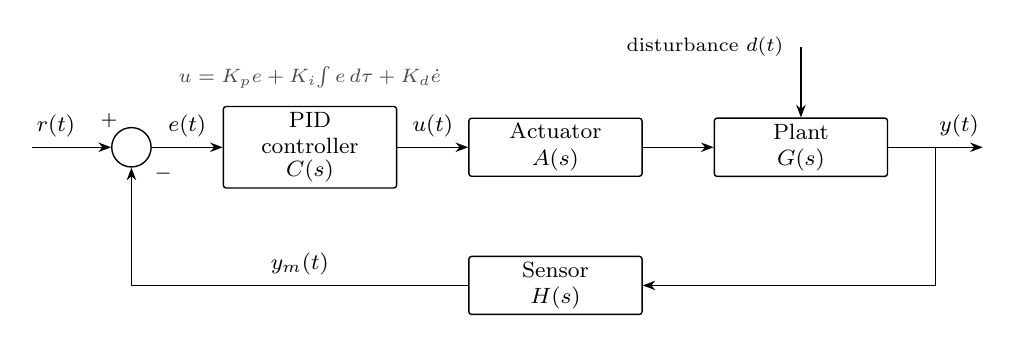
\begin{tikzpicture}[node distance=9mm and 9mm, auto]
  \node[coordinate] (in) {};
  \node[sum, minimum size=5mm, right=10mm of in] (cmp) {};
  \node[block, right=of cmp] (pid) {PID\\controller\\[-1pt]$C(s)$};
  \node[block, right=of pid] (act) {Actuator\\$A(s)$};
  \node[block, right=of act] (plant) {Plant\\$G(s)$};
  \node[coordinate, right=12mm of plant] (out) {};
  \node[block, below=10mm of act] (sens) {Sensor\\$H(s)$};
  \node[coordinate, above=9mm of plant] (dist) {};
  \draw[flow] (in) -- node[pos=0.3] {$r(t)$} (cmp);
  \draw[flow] (cmp) -- node {$e(t)$} (pid);
  \draw[flow] (pid) -- node {$u(t)$} (act);
  \draw[flow] (act) -- (plant);
  \draw[flow] (plant) -- node[pos=0.75] {$y(t)$} (out);
  \draw[flow] ($(plant.east)+(6mm,0)$) |- (sens.east);
  \draw[flow] (sens.west) -| node[pos=0.25, swap] {$y_m(t)$} (cmp.south);
  \draw[flow] (dist) -- (plant.north);
  \node[left=1mm of dist, font=\scriptsize] {disturbance $d(t)$};
  \node[font=\scriptsize] at ($(cmp.north west)+(-1mm,1.5mm)$) {$+$};
  \node[font=\scriptsize] at ($(cmp.south east)+(2.2mm,-1.5mm)$) {$-$};
  \node[above=1mm of pid, font=\scriptsize, text=black!70, align=center]
       {$u=K_p e+K_i\!\int e\,d\tau+K_d\dot e$};
\end{tikzpicture}
}
  \caption{Block diagram of a feedback loop with PID control.}
  \label{fig:loop}
\end{figure}

\begin{figure}[!tbp]
  \centering
  % Step response of a second-order system for several damping ratios,
% plotted natively with PGFPlots (vector, fonts match the document).
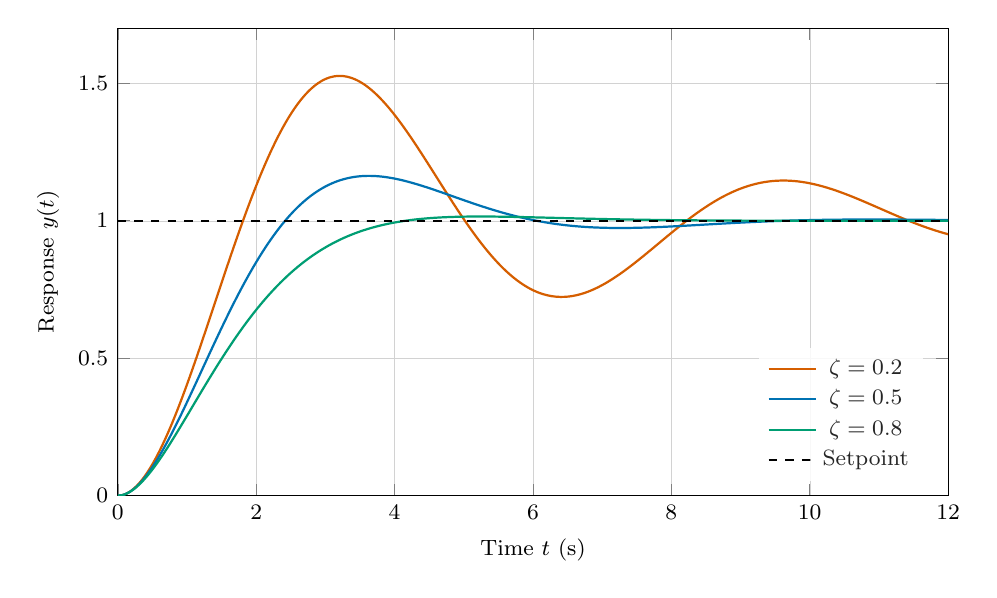
\begin{tikzpicture}
  \begin{axis}[
      width=\linewidth, height=0.62\linewidth,
      xlabel={Time $t$ (s)}, ylabel={Response $y(t)$},
      xmin=0, xmax=12, ymin=0, ymax=1.7,
      grid=both, grid style={line width=.1pt, draw=gray!20}, major grid style={draw=gray!35},
      legend pos=south east, legend style={font=\scriptsize, draw=none, fill=white, fill opacity=0.85},
      every axis plot/.append style={line width=0.8pt}, samples=200, smooth, domain=0:12,
      tick label style={font=\footnotesize}, label style={font=\footnotesize}]
    \def\wn{1}
    \addplot[oiVerm]{1 - exp(-0.2*\wn*x)*(cos(deg(\wn*sqrt(1-0.04)*x)) + (0.2/sqrt(1-0.04))*sin(deg(\wn*sqrt(1-0.04)*x)))};
    \addlegendentry{$\zeta=0.2$}
    \addplot[oiBlue]{1 - exp(-0.5*\wn*x)*(cos(deg(\wn*sqrt(1-0.25)*x)) + (0.5/sqrt(1-0.25))*sin(deg(\wn*sqrt(1-0.25)*x)))};
    \addlegendentry{$\zeta=0.5$}
    \addplot[oiGreen]{1 - exp(-0.8*\wn*x)*(cos(deg(\wn*sqrt(1-0.64)*x)) + (0.8/sqrt(1-0.64))*sin(deg(\wn*sqrt(1-0.64)*x)))};
    \addlegendentry{$\zeta=0.8$}
    \addplot[black, dashed, domain=0:12, samples=2]{1};
    \addlegendentry{Setpoint}
  \end{axis}
\end{tikzpicture}

  \caption{Unit-step response of the second-order model in \cref{eq:plant} for three damping ratios.}
  \label{fig:step}
\end{figure}

\begin{figure}[!tbp]
  \centering
  \resizebox{0.95\columnwidth}{!}{% Finite-state vending controller. Transition labels are placed explicitly
% so the diamond layout remains readable at journal-page scale.
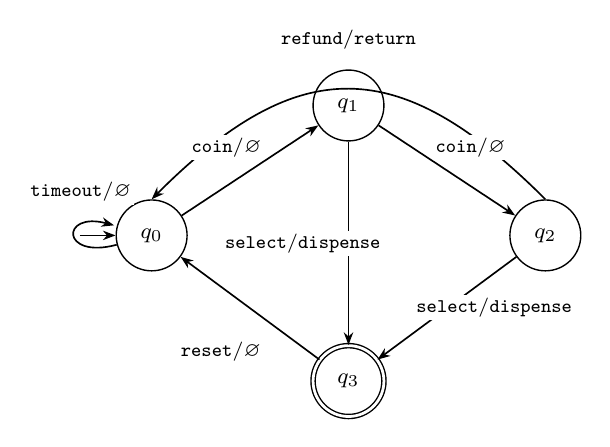
\begin{tikzpicture}[semithick]
  \node[state, initial, initial text=] (s0) at (0,0) {$q_0$};
  \node[state] (s1) at (2.5,1.65) {$q_1$};
  \node[state] (s2) at (5,0) {$q_2$};
  \node[state, accepting] (s3) at (2.5,-1.85) {$q_3$};

  % Transitions
  \path[->]
    (s0) edge[loop left] (s0)
    (s0) edge (s1)
    (s1) edge (s2)
    (s1) edge (s3)
    (s2) edge (s3)
    (s3) edge (s0);
  \draw[->] (s2.north) to[out=135,in=45,looseness=1.35] (s0.north);

  % Explicit labels avoid collisions between converging transitions.
  \node[font=\scriptsize, fill=white, inner sep=1pt] at (-0.9,0.55) {$\mathtt{timeout}/\varnothing$};
  \node[font=\scriptsize, fill=white, inner sep=1pt] at (0.95,1.12) {$\mathtt{coin}/\varnothing$};
  \node[font=\scriptsize, fill=white, inner sep=1pt] at (4.05,1.12) {$\mathtt{coin}/\varnothing$};
  \node[font=\scriptsize, fill=white, inner sep=1pt] at (1.92,-0.10) {$\mathtt{select}/\mathtt{dispense}$};
  \node[font=\scriptsize, fill=white, inner sep=1pt] at (4.35,-0.92) {$\mathtt{select}/\mathtt{dispense}$};
  \node[font=\scriptsize, fill=white, inner sep=1pt] at (0.88,-1.48) {$\mathtt{reset}/\varnothing$};
  \node[font=\scriptsize, fill=white, inner sep=1pt] at (2.5,2.48) {$\mathtt{refund}/\mathtt{return}$};
\end{tikzpicture}
}
  \caption{Example supervisory finite-state machine.}
  \label{fig:fsm}
\end{figure}

\section{Results}\label{sec:results}
The generated dataset contains 2,880 hourly rows from three example sites. Temperature and power have Pearson correlation $r=\rTP$. The hinge regression has in-sample $R^2=\hingeRtwo$. Both values describe this generated dataset; neither measures performance on independent observations.

The four-panel summary is shown in \cref{fig:panels}. Panel \cref{fig:ts} shows daily mean power, \cref{fig:heat} shows pairwise correlations, and \cref{fig:box} compares the generated site distributions. Panel \cref{fig:scat} shows the fitted hinge curve and the dashed linear baseline. The per-site counts, means, and standard deviations appear in \cref{tab:summary}.

\begin{table}[!tbp]
  \centering
  \caption{Summary statistics by example site.}
  \label{tab:summary}
  \sisetup{round-mode=none}
  \input{../../figures/summary_table}
\end{table}

% In standard two-column LaTeX, figure* is a top-of-page float.
\begin{figure*}[!t]
  \centering
  \begin{subfigure}[t]{0.48\textwidth}
    \centering
    \includegraphics[width=\linewidth]{fig_panel_a.pdf}
    \caption{Daily mean power with a one-standard-deviation band.}
    \label{fig:ts}
  \end{subfigure}\hfill
  \begin{subfigure}[t]{0.48\textwidth}
    \centering
    \includegraphics[width=\linewidth]{fig_panel_b.pdf}
    \caption{Correlation matrix.}
    \label{fig:heat}
  \end{subfigure}\\[4pt]
  \begin{subfigure}[t]{0.48\textwidth}
    \centering
    \includegraphics[width=\linewidth]{fig_panel_c.pdf}
    \caption{Power distribution by site.}
    \label{fig:box}
  \end{subfigure}\hfill
  \begin{subfigure}[t]{0.48\textwidth}
    \centering
    \includegraphics[width=\linewidth]{fig_panel_d.pdf}
    \caption{Power against temperature with hinge fit and linear baseline.}
    \label{fig:scat}
  \end{subfigure}
  \caption{Exploratory summaries from the synthetic sensor dataset.}
  \label{fig:panels}
\end{figure*}

The hinge coefficients are solved in closed form by least squares for each candidate threshold. The grid search selects the threshold with the smallest residual sum of squares; the coefficient fit itself does not use an iterative convergence procedure.

\section{Conclusion}
This paper demonstrates a reproducible route from generated CSV data to an IEEE-style PDF. The regression fit, correlation, figures, and table all come from the same synthetic dataset. The controller and step-response diagrams are separate mathematical illustrations. They do not show a controller tested on the data or on a real system.

\bibliographystyle{IEEEtran}
\bibliography{references}
\end{document}
